\chapter{Implementation}\label{chap:implementation}

In this chapter, we describe the main output of this thesis: \textsc{svglab}, a comprehensive Python library for programmatic manipulation of \gls{svg} documents.

The chapter is structured as follows. In Section~\ref{impl:overview}, we provide a brief general overview of the implementation. In Section~\ref{impl:representation}, we describe how the \gls{svg} entities are represented in the library. The parsing and serialization processes are described in Section~\ref{impl:parsing} and Section~\ref{impl:serialization}, respectively. In Section~\ref{reify}, we present our solution to the problem of reification. In Section~\ref{impl:rescaling}, we briefly talk about how we support the rescaling of the coordinate system. Finally, we outline our approach to the calculation of bounding boxes and masks in Section \ref{impl:bbox-mask}.

\section{Overview}\label{impl:overview}

The \textsc{svglab} library is designed as a single Python package of the same name. The package has a flat import structure; all symbols intended for public consumption can be imported directly from the \texttt{svglab} namespace:
\begin{minted}{python}
    from svglab import <symbol>
\end{minted}

The package is compatible with \textsc{CPython}~\cite{python-downloads} versions 3.10 and higher.

The library is designed to comply with the SVG~1.1 specification~\cite{svg11}, supporting all elements and attributes defined thereby. Furthermore, we have incorporated various advantageous features from SVG~2~\cite{svg2} and the SVG~2 Editor's Draft~\cite{svg2-draft}, such as:
\begin{itemize}
    \item the \texttt{pathLength} attribute, present on all basic shapes,
    \item the \texttt{transform-origin} attribute\footnote{See Section~\ref{transform-origin-reify} for more details.}.
\end{itemize}

In total, the library contains the definitions of 80 \gls{svg} elements and 295 attributes.

\section{Representation}\label{impl:representation}

In this section, we describe how our library represents \gls{svg} entities.

Our implementation is capable of representing all types of \gls{svg} entities, ensuring the ability to manipulate \gls{svg} documents in their entirety and that no data is lost between parsing and serialization.

We utilize an object-oriented approach, where each entity type is represented as a class and each entity as an object. We use the \textsc{pydantic}~\cite{pydantic} validation library to construct these classes. This design choice allows us to take advantage of \textsc{pydantic}'s parsing and validation capabilities.

In Figure~\ref{fig:svg-representation}, we show example \gls{svg} code and its \textsc{svglab} representation.

\begin{figure}[H]
  \begin{subfigure}{\textwidth}
    \centering
    \begin{minted}{xml}
        <svg width="200" height="200" xmlns="http://www.w3.org/2000/svg">
          <g id="main-group" fill="blue">
            <rect x="10" y="10" width="50" height="50" stroke="black"/>
            <circle cx="100" cy="50" r="30" stroke="red"/>
            <text x="50" y="150" font-size="18">Hello SVG</text>
          </g>
        </svg>
    \end{minted}
    \caption{SVG source code.}
  \end{subfigure}
  
  \vspace{1cm}
  
  \begin{subfigure}{\textwidth}
    \centering
    \begin{tikzpicture}[
      auto,
      node distance=1.2cm,
      object/.style={
        rectangle split,
        rectangle split parts=2,
        draw,
        fill=white,
        minimum width=4cm,
        text width=3.8cm,
        font=\small
      },
      small-object/.style={
        rectangle split,
        rectangle split parts=2,
        draw,
        fill=white,
        minimum width=3.2cm,
        text width=3cm,
        font=\small
      },
      title/.style={align=center, font=\bfseries},
      svg/.style={object, minimum width=7cm, text width=6.8cm},
      arrow/.style={->, >=Stealth, thick}
    ]
    
    \node[svg] (svg) {
      \nodepart[title]{text}{: Svg}
      \nodepart{second}
      width = Length(200)\\
      height = Length(200)\\
      xmlns = "http://www.w3.org/2000/svg"
    };
    
    \node[object, below=1.5cm of svg] (group) {
      \nodepart[title]{text}{: G}
      \nodepart{second}
      id = "main-group"\\
      fill = Color("blue")
    };
    
    \node[small-object, below left=1.5cm and 0.7cm of group] (rect) {
      \nodepart[title]{text}{: Rect}
      \nodepart{second}
      x = Length(10)\\
      y = Length(10)\\
      width = Length(50)\\
      height = Length(50)\\
      stroke = Color("black")
    };
    
    \node[small-object, below=1.5cm of group] (circle) {
      \nodepart[title]{text}{: Circle}
      \nodepart{second}
      cx = Length(100)\\
      cy = Length(50)\\
      r = 30\\
      stroke = Color("red")
    };
    
    \node[small-object, below right=1.5cm and 0.7cm of group] (text) {
      \nodepart[title]{text}{: Text}
      \nodepart{second}
      x = Length(50)\\
      y = Length(150)\\
      font-size = 18
    };
    
    \node[small-object, below=1.2cm of text] (rawtext) {
      \nodepart[title]{text}{: RawText}
      \nodepart{second}
      content = "Hello SVG"
    };
    
    \draw[arrow] (svg) -- (group);
    \draw[arrow] (group) -- (rect);
    \draw[arrow] (group) -- (circle);
    \draw[arrow] (group) -- (text);
    \draw[arrow] (text) -- (rawtext);
    
    \end{tikzpicture}
    \caption{\textsc{svglab} representation. Arrows indicate parent-child relationships.}
  \end{subfigure}
  \caption{An example SVG and its \textsc{svglab} representation.}
  \label{fig:svg-representation}
\end{figure}

\subsection{Naming}

Our implementation adheres to the naming conventions established by the \gls{svg} specification while adapting them to ensure that all names are valid Python identifiers and that names are better aligned with the Python code style guide~\cite{pep8}. We process the names using the following rules:
\begin{itemize}
    \item all element names are converted to \emph{PascalCase},
    \item attribute names in \emph{kebab-case} are converted to \emph{snake\_case},
    \item attribute names in \emph{camelCase} are kept as-is.
\end{itemize}

If, after this normalization, the resulting name is not a valid Python identifier, we suffix it with an underscore (\,\_\,). Table~\ref{tab:name-normalization} shows several example \gls{svg} names and their normalized versions for use in \textsc{svglab}.

\begin{table}[H]
    \centering
    \begin{tabular}{lll}
        \toprule
        \textbf{Type} & \textbf{\gls{svg} specification} (original) & \textbf{\textsc{svglab}} (normalized) \\
        \midrule
        \multirow{2}{*}{\centering Element} & \texttt{svg} & \texttt{Svg} \\
                & \texttt{rect} & \texttt{Rect} \\
        \midrule
        \multirow{3}{*}{\centering Attribute} & \texttt{stroke-width} & \texttt{stroke\_width} \\
                  & \texttt{viewBox} & \texttt{viewBox} \\
                  & \texttt{class} & \texttt{class\_} \\
        \bottomrule
    \end{tabular}
    \caption{Example element and attribute names and their normalized variants.}
    \label{tab:name-normalization}
\end{table}

\subsection{Entity base classes}\label{impl:representation:abcs}

In this section, we present the \glspl{abc} we use to represent \gls{svg} entities. The hierarchy of these classes is shown in Figure~\ref{fig:entity-hierarchy}.

\begin{figure}[H]
    \centering
    
    \begin{tikzpicture}[
        abstract/.style={draw, rectangle, minimum width=2cm, minimum height=0.7cm, align=center, font=\itshape},
        concrete/.style={draw, rectangle, minimum width=1.5cm, minimum height=0.7cm, align=center},
        inherit/.style={->, >=latex, thick},
        node distance=1.0cm
    ]
        \node[abstract] (Entity) {Entity};
        
        \node[abstract, below left=1cm and 1.2cm of Entity] (CharacterData) {CharacterData};
        \node[abstract, below right=1cm and 1.2cm of Entity] (Element) {Element};
        
        \node[concrete, below left=1cm and 0.1cm of CharacterData] (RawText) {RawText};
        \node[concrete, below=1cm of CharacterData] (Comment) {Comment};
        \node[concrete, below right=1cm and 0.1cm of CharacterData] (CData) {CData};
        
        \node[concrete, below left=1cm and 0.1cm of Element] (G) {G};
        \node[concrete, below=1cm of Element] (Svg) {Svg};
        \node[concrete, below right=1cm and 0.1cm of Element] (Rect) {Rect};
        
        \draw[inherit] (CharacterData) -- (Entity);
        \draw[inherit] (Element) -- (Entity);
        
        \draw[inherit] (RawText) -- (CharacterData);
        \draw[inherit] (Comment) -- (CharacterData);
        \draw[inherit] (CData) -- (CharacterData);
        
        \draw[inherit] (G) -- (Element);
        \draw[inherit] (Svg) -- (Element);
        \draw[inherit] (Rect) -- (Element);
    \end{tikzpicture}
    
    \caption{The entity class hierarchy.}
    \label{fig:entity-hierarchy}
\end{figure}

\subsubsection{Entity}

The base class of the entity hierarchy. This class contains basic attributes and methods common to all entities, such as \texttt{parent}, a reference to the parent element, or \texttt{to\_xml()}, a method that serializes the entity to its \gls{svg} representation.

\subsubsection{Element}

The base class for all \gls{svg} elements, which contains additional attributes and methods specific to elements in \gls{svg}. These include \texttt{children}, \texttt{descendants}, \texttt{siblings}, \texttt{find()}, and \texttt{find\_all()}, which are attributes and methods for navigating the entity tree. It also includes \texttt{add\_child()}, \texttt{remove\_child()}, and \texttt{clear\_children()}, which are methods to manipulate the entity tree.

For each concrete \gls{svg} element, we create an \emph{element class} (such as \texttt{Svg} or \texttt{Rect}), which inherits from the \texttt{Element} class.

\subsubsection{CharacterData}

The base class for textual entities in \gls{svg}. It contains only one attribute: \texttt{content}, which stores the raw textual content of the entity. 
    
For each concrete \gls{svg} textual entity, we create a class that inherits from \texttt{CharacterData}: the classes \texttt{Comment}, \texttt{CData}, and \texttt{RawText} represent comments, CDATA sections, and text, respectively.

\subsection{Attributes}

For the purposes of our implementation, we divide the element attributes into two categories:
\begin{itemize}
    \item \emph{standard attributes}: all attributes defined in any of the \gls{svg} specifications,
    \item \emph{extra attributes}: all other, user-defined attributes.
\end{itemize}

We offer first-class support for standard attributes: they are represented as native Python objects for convenient manipulation, and they are automatically parsed and validated. In contrast, we store extra attributes in their original string form. By storing non-standard attributes, we ensure that our implementation complies with the requirement that no data is lost between parsing and serialization.

In this section, we will describe our approach to representing standard attributes. We represent simple attributes such as numbers, strings, and booleans using the appropriate standard Python types. For more complex attributes such as lengths, colors, transformations, and path data, we define custom dataclasses.

\subsubsection{Lengths and angles}

For the \texttt{length} and \texttt{angle} types, we provide the \texttt{Length} and \texttt{Angle} classes, respectively. Both classes provide comparable functionality and have a similar interface. The classes contain the following attributes:
\begin{itemize}
    \item \texttt{value}: the floating-point value of the quantity (length or angle), e.g. \texttt{45},
    \item \texttt{unit}: the unit associated with the quantity, e.g. \texttt{"deg"}.
\end{itemize}

The classes also define a \texttt{to(unit)} method which returns a new object of the same type, but with the value converted to the specified unit. If conversion is not possible, an exception is raised.

We use operator overloading to define the operations of addition ($+$) and subtraction ($-$) on two lengths (or two angles):
\begin{minted}{python}
    a = Length(1, "cm")
    b = Length(5, "mm")
    c = a + b  # Length(1.5, "cm")
\end{minted}

If the units of the operands differ, the result is returned in the units of the left operand.

We also support the multiplication (*) and division (/) of lengths and units by scalars:
\begin{minted}{python}
    a = Angle(45, "deg")
    b = 2 * a  # Angle(90, "deg")
\end{minted}

\subsubsection{Points}

To represent the \texttt{points} type, we have created the \texttt{Point} class to represent a point in the plane\footnote{We also use this class to represent vectors in two-dimensional space. Although we acknowledge the formal distinction between points and vectors, we do not provide a dedicated class for manipulating vectors, as its implementation would be virtually identical to the \texttt{Point} class.}. The class contains two attributes:
\begin{itemize}
    \item \texttt{x}: the $x$-coordinate of the point,
    \item \texttt{y}: the $y$-coordinate of the point.
\end{itemize}

We support the operations of addition ($+$) and subtraction ($-$) of two points and multiplication (*) and division (/) by a scalar:
\begin{minted}{python}
    a = Point(1, 1)
    b = Point(1, 0)
    c = a + 2 * b  # Point(3, 1)
\end{minted}

The \texttt{Points} type is then constructed simply as a list of points (that is, type \py{list[Point]}).

\subsubsection{Transformations}

We represent each type of \gls{svg} transformation using an associated class. The classes are listed in Table~\ref{tab:transformation-classes}.

\begin{table}[H]
    \centering
    \begin{tabular}{lll}
    \toprule
    \textbf{\gls{svg} syntax} & \textbf{\textsc{svglab} class} & \textbf{Attributes} \\
    \midrule
    $\operatorname{translate}\left(t_x, t_y\right)$ & \texttt{Translate} & \texttt{tx}, \texttt{ty} \\
    $\operatorname{scale}\left(s_x, s_y\right)$ & \texttt{Scale} & \texttt{sx}, \texttt{sy} \\
    $\operatorname{rotate}\left(\alpha, c_x, c_y\right)$ & \texttt{Rotate} & \texttt{angle}, \texttt{cx}, \texttt{cy} \\
    $\operatorname{skewX}\left(\alpha\right)$ & \texttt{SkewX} & \texttt{angle} \\
    $\operatorname{skewY}\left(\alpha\right)$ & \texttt{SkewY} & \texttt{angle} \\
    $\operatorname{matrix}\left(a, b, c, d, e, f\right)$ & \texttt{Matrix} & \texttt{a}, \texttt{b}, \texttt{c}, \texttt{d}, \texttt{e}, \texttt{f} \\
    \bottomrule
    \end{tabular}
    \caption{Representation of SVG transformations in \textsc{svglab}.}
    \label{tab:transformation-classes}
\end{table}

Instances of each class can be converted to equivalent instances of type \texttt{Matrix} using the \texttt{to\_matrix()} method:
\begin{minted}{python}
    t = Translate(1, 2)
    m = t.to_matrix()  # Matrix(0, 0, 0, 0, 1, 2)
\end{minted}

Transformations may be composed using the matrix multiplication operator (@):
\begin{minted}{python}
    a = Translate(1, 2)
    b = Scale(3, 4)
    c = a @ b  # Matrix(3, 0, 0, 4, 1, 2)
\end{minted}
Similarly, transformations can be applied to points:
\begin{minted}{python}
    a = Point(1, 0)
    b = Translate(0, 2)
    c = b @ a  # Point(1, 2)
\end{minted}

The \texttt{transform-list} type is then a list of any of the transformation classes, that is, 
\begin{minted}{python}
   list[Translate | Scale | Rotate | SkewX | SkewY | Matrix] 
\end{minted}

\subsubsection{Colors}

For representing colors, we provide a \texttt{Color} class\footnote{Most of the functionality is provided by the \textsc{pydantic-extra-types}~\cite{pydantic-extra-types} package.}. Objects of type \texttt{Color} are initialized using the string representation of the color: \texttt{"rgb(255, 0, 0)"}, for instance. The class provides methods such as \texttt{as\_hsl()} and \texttt{as\_named()} that return the string representation of the color in the desired format.

\subsubsection{Path data}

Our approach to representing path data is similar to that used to represent transformations. For each path command, we provide an associated class. Table~\ref{tab:path-commands} shows each type of command and the class that we use to represent it.

\begin{table}[H]
    \centering
    
    \begin{tabular}{c p{5cm} l}
        \toprule
        \textbf{Cmd.} & \textbf{Name} & \textbf{\textsc{svglab} class} \\
        \midrule
        \textbf{M} & moveto & \texttt{MoveTo} \\
        \textbf{Z} & closepath & \texttt{ClosePath} \\ \hline
        \textbf{L} & lineto & \texttt{LineTo} \\
        \textbf{H} & horizontal lineto & \texttt{HorizontalLineTo} \\
        \textbf{V} & vertical lineto & \texttt{VerticalLineTo} \\ \hline
        \textbf{C} & curveto & \texttt{CubicBezierTo} \\
        \textbf{S} & shorthand\slash smooth curveto & \texttt{SmoothCubicBezierTo} \\ \hline
        \textbf{Q} & quadratic Bézier curveto & \texttt{QuadraticBezierTo} \\
        \textbf{T} & shorthand\slash smooth quadratic Bézier curveto & \texttt{SmoothQuadraticBezierTo} \\ \hline
        \textbf{A} & elliptical arc & \texttt{ArcTo} \\
        \bottomrule
    \end{tabular}
    
    \caption{Path commands and their representations in \textsc{svglab}.}
    \label{tab:path-commands}
\end{table}

As mentioned in Section~\ref{theo:svg}, the commands \textbf{H}, \textbf{V}, \textbf{S}, and \textbf{T} are \emph{shorthand commands}, and the values of some of their parameters are inferred from the context. In our implementation, this calculation is performed solely on an as-needed basis. Notably, no Python package appears to support shorthand commands at the time of writing; instead, existing implementations resolve shorthand commands to their full versions upon parsing~\cite{svgelements, svgpathtools, regebro2013svgpath}.

The path data as a whole is represented by the \texttt{PathData} class. It is a mutable sequence\footnote{In other words, the class inherits from \texttt{collections.abc.MutableSequence}.} of path commands and can be used as the value of the \texttt{d} attribute for the \texttt{<path>} element. The \texttt{PathData} class contains sanity checks to ensure that the path is always valid. For example, the first command of the path must be a \texttt{MoveTo} command.

Similarly to points, transformations may be applied to path data:
\begin{minted}{python}
    path = PathData()
            .line_to(Point(1, 1))
            .quadratic_bezier_to(Point(5, 0), Point(10, 10))
            .close()
    SkewX(30) @ path  # PathData(...)
\end{minted}

Path commands can be incorporated into the path data via methods from the \texttt{MutableSequence} \gls{abc}, such as \texttt{append()}, or using convenience methods defined in the \texttt{PathData} class, such as \py{PathData.line_to()}.

By default, command coordinates are interpreted as absolute. However, the user may also wish to specify commands using relative coordinates. This can be done using the aforementioned methods with \py{relative=True}.

The \pathcommand{ClosePath}{Z} command deserves particular attention---it is the only command that requires no parameters and thus requires specialized handling.

Existing libraries (such as \textsc{svgpathtools} \cite{svgpathtools}) sometimes implement this feature by treating the command as if it were a line. When the user manipulates the path containing the said command and subsequently attempts to serialize it, the library outputs \textbf{Z} if the endpoint of the \pathcommand{LineTo}{L} command coincides with the starting point of the path, \textbf{L} otherwise. This approach produces incorrect results (see Figure~\ref{fig:close-path-incorrect}) because the information on whether the path is closed is irrevocably lost during this conversion.

To avoid this issue, we instead represent the command as is, using a dedicated class. We can use this approach because no matter which affine transformations we apply to our path, the transformed path will be closed precisely when the original path was closed (see Theorem~\ref{closed-path-composition} for proof).

\subsubsection{Attribute composition}\label{impl:representation:attr-composition}

We use primitive Python types and the dataclasses described above to define attributes. Each attribute is defined using a mixin class; for instance:
\begin{minted}{python}
    class StrokeWidthAttr:
        stroke_width: Length | Literal[
            "none",
            "inherit"
        ] | None = None
\end{minted}

These mixin classes, along with the \texttt{Element} \gls{abc}, are then combined to form a final concrete element class, such as \texttt{Rect}:
\begin{minted}{python}
    class Rect(StrokeWidthAttr, Element):
        pass
\end{minted}

This approach has the following benefits:
\begin{itemize}
    \item simple composition of attribute classes into element classes without redundancy,
    \item the possibility to share attribute documentation,
    \item 
    \begin{samepage}
    the possibility to determine the presence of an attribute on an element in a type-safe manner via \texttt{isinstance()}:
    \begin{minted}{python}
        elem = ...
        elem.stroke_width = Length(10)  # type checker error
        
        if isinstance(elem, StrokeWidthAttr):
            elem.stroke_width = Length(10)  # OK
    \end{minted}
    \end{samepage}
\end{itemize}

The concept is depicted in Figure~\ref{fig:element-composition}.

\begin{figure}[H]
    \centering
    \begin{tikzpicture}[
        node distance=0.7cm,
        box/.style={draw, minimum width=2cm, minimum height=0.7cm, align=center},
        line/.style={thick}
    ]
        \node[box] (strokewidth) at (0,2) {StrokeWidthAttr};
        \node[box] (class) at (0,1) {ClassAttr};
        \node[box] (id) at (0,0) {IdAttr};
        \node[box] (x) at (0,-1) {XAttr};
        \node[box] (y) at (0,-2) {YAttr};
        
        \path (strokewidth.center) -- (y.center) coordinate[midway] (midpoint);
        \node[box] (rect) at (5,0) {Rect};
        \coordinate (merge) at (3.75,0);
        
        \draw[line] (strokewidth.east) .. controls +(right:2cm) and +(left:1cm) .. (merge);
        \draw[line] (class.east) .. controls +(right:1.5cm) and +(left:0.8cm) .. (merge);
        \draw[line] (id.east) -- (merge);
        \draw[line] (x.east) .. controls +(right:1.5cm) and +(left:0.8cm) .. (merge);
        \draw[line] (y.east) .. controls +(right:2cm) and +(left:1cm) .. (merge);
        
        \draw[-{Stealth[length=3mm]}, thick] (merge) -- (rect.west);
    \end{tikzpicture}
    \caption{The composition of attribute mixin classes into an element class.}
    \label{fig:element-composition}
\end{figure}

The element classes themselves typically do not contain any additional logic or attribute definitions. Where appropriate, we group several attributes often used together into a single mixin class.

\subsection{Traits}

In the \gls{svg} specification~\cite{svg11}, elements that are related in some way are often referred to by a special term. Such groups of elements include \emph{graphics elements}, \emph{shapes}, and \emph{basic shapes}, which we have introduced in Section~\ref{theo:svg}. Another example is the \emph{container elements}: elements that may contain other elements as children~\cite[Sec.~1.6]{svg11}. 

For each of the groups defined in~\cite[Sec.~1.6]{svg11}, we create an \gls{abc}; collectively, we call these \glspl{abc} \emph{traits}. Elements pertaining to a particular group inherit the associated trait.

\begin{samepage}
We do this because elements belonging to the same group can often share common attributes or functionality; for instance, the operation of calculating a bounding box is defined on all graphics elements:
\begin{minted}{python}
    class GraphicsElement(...):
        def get_bbox() -> Bbox:
            ...
\end{minted}
\end{samepage}

\begin{samepage}
This approach allows us to further reduce code duplication when defining elements. In addition, it allows users to conveniently check elements against familiar terminology used in the \gls{svg} specification:
\begin{minted}{python}
    elem = Rect()
    isinstance(elem, BasicShape)        # True
    isinstance(elem, ContainerElement)  # False
\end{minted}
\end{samepage}

\section{Elements}

We represent \gls{svg} elements using \textsc{pydantic}~\cite{pydantic} models. As described in Section~\ref{impl:representation:attr-composition}, we compose previously defined attribute mixin classes into \emph{element classes}, where each distinct \gls{svg} element has a corresponding class. Examples include \texttt{Svg}, \texttt{Rect}, \texttt{Circle}, or \texttt{Path}. 

All \emph{standard attributes} can be accessed and modified using dot notation and passed to the constructor:
\begin{minted}{python}
    rect = Rect(x=Length(10), color=Color("black"))
    rect.color = Color("#ff00ff")
    rect.x  # Length(10)
    rect.y  # None
\end{minted}

By default, all attribute values are initialized to \py{None}. The value of \py{None} signifies the absence of an attribute; attributes with this value will not be included in the serialized output:
\begin{minted}{python}
    rect = Rect()
    rect.to_xml()  # <rect />
\end{minted}

Non-standard attributes (or \emph{extra attributes}) may also be passed to the constructor, but their type must be \py{str}. Instead of using the dot notation, they are available as a dictionary of type \py{dict[str, str]}:
\begin{minted}{python}
    Circle(foo=1)               # error, must be str
    circ = Circle(foo="bar")    # OK
    circ.extra_attrs()          # {"foo": "bar"}
\end{minted}

\section{Parsing}\label{impl:parsing}

In this section, we describe how we parse \gls{svg} documents from their textual representation into their \textsc{svglab} representation we described in the previous section.

Our mechanism for parsing an \gls{svg} document is fundamentally divided into the following two stages:
\begin{enumerate}
    \item \label{parsing-1} parsing the \gls{svg} document with an \gls{xml} parser to obtain an entity tree,
    \item \label{parsing-2} parsing the attributes of each element in the tree into native Python types.
\end{enumerate}

We delegate the \hyperref[parsing-1]{initial phase} to \textsc{Beautiful Soup}~\cite{beautifulsoup4}, a Python toolkit designed to parse \gls{html} and \gls{xml} documents. First, we use \textsc{Beautiful Soup} to parse the \gls{svg} document into a tree of \textsc{Beautiful Soup} objects. In \hyperref[parsing-2]{stage two}, we transform these objects into instances of \textsc{svglab} classes such as \texttt{Svg} and \texttt{Rect}, parsing the attributes along the way. The entire process is depicted in Figure~\ref{fig:parsing-serialization-process}.

\begin{figure}[H]
    \centering
    \begin{tikzpicture}[
        node distance=2cm,
        box/.style={rectangle, draw, text width=5cm, text centered, minimum height=1cm, rounded corners},
        arrow/.style={thick, -Stealth},
        process/.style={ultra thick, -Stealth}
    ]

    \node[box] (svg) {\acrshort{svg} document};
    \node[box, below=of svg] (bs) {\textsc{Beautiful Soup} object};
    \node[box, below=of bs] (lib) {\textsc{svglab} object};
    
    \draw[arrow] ([xshift=-2cm]svg.south) -- node[midway, fill=white, inner sep=2pt] {parse with \textsc{B}.~\textsc{S}.} ([xshift=-2cm]bs.north);
    \draw[arrow] ([xshift=-2cm]bs.south) -- node[midway, fill=white, inner sep=2pt] {parse attributes} ([xshift=-2cm]lib.north);
    
    \draw[arrow] ([xshift=2cm]lib.north) -- node[midway, fill=white, inner sep=2pt] {serialize attributes} ([xshift=2cm]bs.south);
    \draw[arrow] ([xshift=2cm]bs.north) -- node[midway, fill=white, inner sep=2pt] {serialize with \textsc{B}.~\textsc{S}.} ([xshift=2cm]svg.south);

    \coordinate (nw) at ([xshift=-1.5cm]current bounding box.north west);
    \coordinate (sw) at ([xshift=-1.5cm]current bounding box.south west);
    \coordinate (ne) at ([xshift=1.5cm]current bounding box.north east);
    \coordinate (se) at ([xshift=1.5cm]current bounding box.south east);

    \draw[process] (nw) -- node[midway, fill=white, inner sep=2pt] {\textbf{Parsing}} (sw);
    \draw[process] (se) -- node[midway, fill=white, inner sep=2pt] {\textbf{Serialization}} (ne);

    \end{tikzpicture}
    \caption{The parsing and serialization processes.}
    \label{fig:parsing-serialization-process}
\end{figure}

Most attribute values represent basic types\footnote{For instance, string literals, numbers, boolean values, and unions and sequences thereof.} and therefore can be parsed directly by \textsc{Pydantic}.

However, \gls{svg} contains several more elaborate attribute types, such as \texttt{length} or \texttt{angle}. We must parse those attributes manually.

To accomplish this task, we use the \textsc{Lark}~\cite{lark} parser generator. With a context-free grammar specified using \textsc{Lark}'s grammar language, similar to \gls{ebnf}, \textsc{Lark} can parse arbitrary input into Python objects~\cite{lark-docs}.

A parser generator enables robust and maintainable attribute parsing compared to traditional methods, such as manually constructing a recursive-descent parser.

\subsection{\textsc{Beautiful Soup} parsers}

The \textsc{Beautiful Soup} library offers the option to use several different parsers~\cite{beautifulsoup4}:

\begin{itemize}
    \item \texttt{html.parser}: an \gls{html} parser with medium performance that is a part of the Python standard library,
    \item \texttt{lxml}: an \gls{html} parser with high performance; requires an external dependency (\textsc{lxml}~\cite{lxml}),
    \item \texttt{lxml-xml}: an \gls{xml} parser with high performance; requires an external dependency (\textsc{lxml}),
    \item \texttt{html5lib}: an extremely lenient \gls{html} parser with very low performance; requires an external dependency (\textsc{html5lib}~\cite{html5lib}).
\end{itemize}

We use the \texttt{lxml-xml} parser because it is purpose-built for \gls{xml} parsing, offers superior performance, and is recommended for general use by the \textsc{Beautiful Soup} documentation~\cite{beautifulsoup4}. Users may opt for an alternative parser if preferred---our implementation is designed to ensure uniform behavior across different parsers.

\subsection{Using HTML parsers}

Although \gls{html} parsers generally work well for parsing \gls{svg} documents, they automatically enclose the document in varying \gls{html} elements such as \texttt{<html>} and \texttt{<body>}. 

To overcome this limitation, we perform a \gls{bfs} of the parsed tree to locate the outermost \texttt{<svg>} element. If found, the element is considered the root \gls{svg} document fragment and designated the root of the \gls{svg} element tree. If there is no such element or if one of the element's siblings is an \texttt{<svg>} element (and so there is more than one root \texttt{<svg>} element), the input is assumed invalid.

As a corollary, this approach enables the parsing of \gls{svg} embedded in \gls{html} documents.

\section{Serialization and output formatting}\label{impl:serialization}

In this section, we describe serialization, the process of converting library objects into their string representation. 

Recall Figure~\ref{fig:parsing-serialization-process} and notice that the serialization process is precisely the opposite of the parsing method we have described in the previous section.

The library supports a wide range of configurable formatting rules that can be applied during serialization. We describe some of those as well.

\subsection{The formatter}

To facilitate the user's ability to customize the formatting options, we have created a dataclass called \texttt{Formatter}. 

The user can utilize the formatter to specify their desired formatting preferences. Subsequently, the formatter can be used in several ways (from lowest to highest priority):
\begin{itemize}
    \item globally using the \texttt{set\_formatter()} function,
    \item temporarily using a context manager,
    \item as a direct argument supplied to functions that output \gls{xml} (such as \texttt{to\_xml()}).
\end{itemize}

The formatter contains, among others, the following options:
\begin{itemize}
    \item \py{indent: int} \\
    the number of spaces to use for indentation,
    \item \py{path_data_commands: "implicit" | "explicit"} \\
    whether to use implicit or explicit commands in path data,
    \item \py{path_data_coordinates: "absolute" | "relative"} \\
    whether to use absolute or relative coordinates in path data,
    \item \py{alpha_channel: "percentage" | "float"} \\
    whether to represent the alpha channel of colors as a percentage (e.g., 50\%) or a decimal number from the interval $\interval[scaled]{0}{1}$ (e.g., 0.5).
\end{itemize}

In total, the formatter supports 24 formatting directives.

\subsection{Serializable objects}

Not all Python objects are serializable. Serializable objects include a small set of predefined primitives and objects that implement the \texttt{CustomSerializable} protocol. Moreover, iterables of serializable objects also form a serializable object.

\subsection{Serialization of primitives}

Certain primitive types are serialized directly in the \texttt{serialize()} function due to their inability to implement the \texttt{CustomSerializable} protocol. They are:

\begin{itemize}
    \begin{samepage}
    \item \py{int}\quad
    \item \py{float}\quad \smash{\raisebox{.5\dimexpr\baselineskip+\itemsep+\parskip}{
        $\left.\rule{0pt}{.5\dimexpr2\baselineskip+\itemsep+\parskip}\right\}$
          serialized using several user-defined formatting rules,}}
    \end{samepage}
    \item \py{str}\quad serialized as-is,
    \item \py{bool}\quad serialized as \py{"false"} and \py{"true"} or \py{"0"} and \py{"1"}, depending on the context.
\end{itemize}

Serialization is performed by a set of mutually recursive functions. For example, the \texttt{serialize()} function serializes iterables by recursively calling itself on each item in the iterable and joining the results.

\subsection{The \texttt{CustomSerializable} protocol}

The \texttt{CustomSerializable} protocol is a simple protocol that requires the implementation of a single method:
\begin{minted}{python}
    class CustomSerializable(Protocol):
        def serialize(self) -> str:
            ...
\end{minted}

The protocol allows arbitrary objects to define their own serialization logic. As an example, consider the \texttt{Point} class:

\begin{minted}{python}
    class Point(CustomSerializable, ...):
        ...

        @override
        def serialize(self) -> str:
            formatter = serialize.get_current_formatter()
            x, y = serialize.serialize(self.x, self.y)

            return f"{x}{formatter.point_separator}{y}"
\end{minted}

In this example, \py{get_current_formatter()} retrieves the current formatting settings. Then, the \texttt{serialize()} function serializes two floats, the $x$ and $y$ coordinates of the point. Subsequently, these coordinates are combined according to user preferences to produce the final string representation. This example illustrates how predefined and custom serialization logic is combined to form a coherent serialization model.

\subsection{The serialization process}

With these principles established, we can analyze the logic of \texttt{serialize()}, the core of the serialization process. The function takes an arbitrary object and, using the current formatter settings, returns the object's string representation.

Initially, the function ensures that the object is serializable. Should the value be one of the predefined primitives, it is serialized directly using the appropriate function. In instances where the object implements the \texttt{CustomSerializable} protocol, its \texttt{serialize()} method is invoked, and the result is returned. As a special case, if the object is iterable, its values are serialized using a recursive call to \texttt{serialize()} and thereafter combined.

\section{Reification}\label{reify}

In this section, we present our implementation of the reification algorithm. Our objective is to systematically process the transformation lists of elements and apply the transformations found therein to the elements' attributes. In doing so, the transformations will effectively become \emph{baked into} the attributes of the elements. At the end of the process, the \texttt{transform} attributes can be safely removed. As an example, consider the following \gls{svg} code:
\begin{minted}{xml}
    <svg width="100" height="100">
      <g transform="translate(25, 50) scale(2)">
        <rect x="5" y="5" width="10" height="5" transform="translate(5, 10)" />
      </g>
    </svg>
\end{minted}

In this \gls{svg} document, we have two elements with associated transformation lists. We wish to obtain the following (visually equivalent) \gls{svg} where all transformations have been reified:
\begin{minted}{xml}
    <svg width="100" height="100">
      <g>
        <rect x="45" y="80" width="20" height="10" stroke-width="2" />
      </g>
    </svg>
\end{minted}

Let us begin with the observation that not all transformations can be reified.

\subsection{Non-reifiable transformations}

Not all transformations can be reified because of their effect on the element's stroke. Consider, for instance, an element with the non-uniform scaling transformation
    \[
        \operatorname{scale}(2, 1)
    \]
applied to it. This transformation creates a stroke of unequal width along the $x$ and $y$ axes, as demonstrated in Figure~\ref{fig:non-uniform-scale-rect}.
\begin{figure}[H]
    \centering
    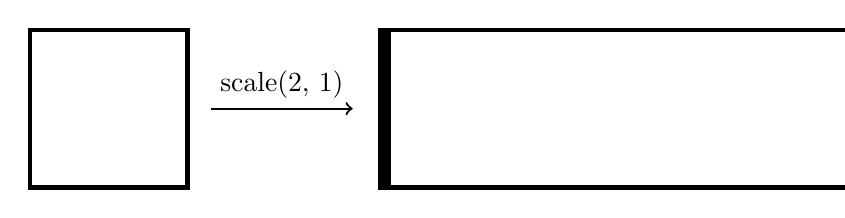
\begin{tikzpicture}[ultra thick]
        \draw (0, 0) rectangle (2,2);
        \draw[transform canvas={xscale=3},xshift=-2.5cm] (4, 0) rectangle (6,2);
        \draw[->, thick] (2.3, 1) -- (4.1, 1) node[midway, above] {scale(2, 1)};
        \useasboundingbox (0, 0) rectangle (10, 2); % bounding box fix
    \end{tikzpicture}
    \caption{The effect of non-uniform scaling on a shape's stroke.}
    \label{fig:non-uniform-scale-rect}
\end{figure}
Recall now that in \gls{svg}, the width of the stroke is specified by the \texttt{stroke-width} attribute, in which a single value determines the thickness of the stroke along the entire outline of the element. Clearly, the \texttt{stroke-width} attribute does not offer a means to represent the non-uniform stroke width on our transformed element. Therefore, it is not possible to represent the transformed element using the syntax of \gls{svg}\footnote{Technically, it may be possible to represent this shape using paths. However, determining the correct path data to represent the transformed element would be far from trivial (especially when a skewing transformation is applied). Furthermore, this approach would typically increase the overall size and complexity of the document, which would largely defeat the purpose of reification.}. Similarly, skewing transformations may not be reified for the same reason.

Furthermore, the reified shape may not always be representable using the original \gls{svg} element. For example, reifying rotation on a rectangle without converting it to an equivalent path is not possible. Table~\ref{table:reification-possibility} shows which transformations are reifiable on different \gls{svg} shapes.

\begin{table}[H]
    \centering

    \begin{threeparttable}
        \begin{tabular}{lcccc}
          \toprule
          & $\operatorname{translate}()$ & $\operatorname{scale}()$ & $\operatorname{rotate}()$ & $\operatorname{skewX}()$ and $\operatorname{skewY()}$ \\
          \midrule
          \texttt{<line>} & \picheckmark & \picheckmark & \picheckmark & \picrossmark \\
          \texttt{<rect>} & \picheckmark & \picheckmark & \picross & \picrossmark \\
          \texttt{<circle>} & \picheckmark & \picheckmark & \picheckmark & \picrossmark \\
          \texttt{<ellipse>} & \picheckmark & \picheckmark & \picross & \picrossmark \\
          \texttt{<polygon>} & \picheckmark & \picheckmark & \picheckmark & \picrossmark \\
          \texttt{<polyline>} & \picheckmark & \picheckmark & \picheckmark & \picrossmark \\
          \texttt{<path>} & \picheckmark & \picheckmark & \picheckmark & \picrossmark \\
          \bottomrule
      \end{tabular}
    
      \begin{tablenotes}
          \item[\picheckmark] Possible to reify.
          \item[\picross] Possible to reify only after converting the element to a path.
          \item[\picrossmark] Not possible to reify.
      \end{tablenotes}

      \caption{The possibility of reification among different types of elements and~transformations.}
      \label{table:reification-possibility}
    \end{threeparttable}
\end{table}

\subsection{Reordering transformations} \label{reordering-transformations}

Affine transformations are inherently non-commutative; the order in which they are applied significantly impacts the resulting shape. Given a transformation list
\[
    T_1\, T_2\, \ldots\, T_n\text{,}
\]
only the last transformation $T_n$ can be applied directly to the element. Consequently, encountering a non-reifiable transformation during reification requires the reification process to halt, which leaves that transformation and any subsequent transformations in the list.

To address this limitation, we propose to reorder the transformations such that all non-reifiable transformations occur first in the list, followed by transformations that can be reified. This method enables the reification of all but the non-reifiable transformations---regardless of their position within the original list. That is, given a transformation list $L$, consisting of reifiable transformations $T_1 \ldots T_n$ and non-reifiable transformations $N_1 \ldots N_k$, we want to find a new list $L'$ such that
\[
    L' = N_1\,N_2\,\ldots\,N_k\,T_1\,T_2\,\ldots\,T_n
\]
and
\[
    \prod_{t \in L}{t} = \prod_{s \in L'}{s}\text{.}
\]

To tackle the task of reordering affine transformations, we have derived the following identities (see Appendix~\ref{appx:proofs-and-derivations} for the derivations):
\begin{gather}
    \operatorname{translate}\left(t_x, t_y\right)\operatorname{scale}\left(s_x, s_y\right) = \operatorname{scale}\left(s_x, s_y\right)\operatorname{translate}\left(\frac{t_x}{s_x}, \frac{t_y}{s_y}\right) \\
    \operatorname{translate}\left(t_x, t_y\right)\operatorname{skewX}(\alpha) = \operatorname{skewX}(\alpha)\operatorname{translate}\left(t_x - t_y \tan{\alpha}, t_y\right) \\
    \operatorname{translate}\left(t_x, t_y\right)\operatorname{skewY}(\alpha) = \operatorname{skewY}(\alpha)\operatorname{translate}\left(t_x, t_y - t_x\tan{\alpha}\right) \\
    \operatorname{scale}\left(s_x, s_y\right)\operatorname{skewX}(\alpha) = \operatorname{skewX}\left(\arctan\left(\frac{s_x}{s_y} \tan{\alpha}\right)\right)\operatorname{scale}\left(s_x, s_y\right) \\
    \operatorname{scale}\left(s_x, s_y\right)\operatorname{skewY}(\alpha) = \operatorname{skewY}\left(\arctan\left(\frac{s_y}{s_x} \tan{\alpha}\right)\right)\operatorname{scale}\left(s_x, s_y\right) \\
    \operatorname{translate}\left(t_x, t_y\right)\operatorname{rotate}\left(\alpha, c_x, c_y\right) = \operatorname{rotate}\left(\alpha, c_x + t_x, c_y + t_y\right) \\
    \operatorname{scale}\left(s_x, s_y\right)\operatorname{rotate}\left(\alpha, c_x, c_y\right) = \operatorname{rotate}\left(\alpha, s_x \cdot c_x, s_y \cdot c_y\right)\operatorname{scale}\left(s_x, s_y\right)
\end{gather}

In each formula, the transformations are swapped and their parameters are adjusted so that the effect of composing the transformations remains unaltered.

\subsection{Decomposition of affine transformation matrices into elementary transformations} \label{matrix-decomposition}

As discussed in section~\ref{reordering-transformations}, swapping the order of two transformations is crucial in the reification process. We have shown that for pairs of \emph{elementary transformations} (\texttt{translate}, \texttt{scale}, \texttt{rotate}, \texttt{skewX}, and \texttt{skewY}), there exist formulas that allow their orders to be swapped and their parameters adjusted in a manner that preserves the overall effect when the transformations are composed. 

However, we hypothesize that there is no simple closed-form formula for arbitrary affine transformations of the form \texttt{matrix(a, b, c, d, e, f)}.

To address this limitation, we propose decomposing all matrices in a transform list as a preprocessing step before reification begins. Let $T$ be an affine transformation given in homogeneous coordinates:
\[
    T = 
    \begin{pmatrix}
        a & c & e \\
        b & d & f \\
        0 & 0 & 1
    \end{pmatrix}
    \text{.}
\]
Using the definition of an affine transformation $T\left(x\right) \coloneqq Ax + \vec{b}$ allows us to isolate the translation vector $\vec{b} = \vector{e, f}^T$ and proceed with the decomposition of the linear transformation $A$:
\[
    T\left(x\right) = Ax + \vec{b} =
    \begin{pmatrix}
        a & c \\
        b & d \\
    \end{pmatrix}
    x +
    \begin{pmatrix}
        e \\
        f
    \end{pmatrix}
    \text{.}
\]
We want to obtain a factorization of $A$ such that each factor contains only one type of elementary transformation.

According to \textcite{wang2013decomposition}, the \gls{ldu} and QR factorizations form promising candidates for a suitable decomposition. However, neither method is universally optimal in the sense that the decomposition may occasionally contain \enquote{undesirable} transformation types (skewing, non-uniform scaling), even though the transformation could be expressed without them (for example, using rotation). In this regard, \gls{ldu} is unsuitable for matrices that involve rotation (but handles skewing well), while QR struggles with skewing (and, in contrast to \gls{ldu}, handles rotation well)~\cite{wang2013decomposition}.

Therefore, we propose a hybrid approach that involves computing both factorizations and selecting the most suitable one. The selection is made using a cost function $\omega$, defined as:
\[
    \omega(t) = 
    \begin{cases}
        10^6 & \text{if $t$ is a skew or non-uniform scale,} \\
        10^3 & \text{if $t$ is a rotation,} \\
        1 & \text{otherwise.}
    \end{cases}
\]
The costs are defined in a manner that avoids non-reifiable transformations and favors simpler decompositions. The cost of a decomposition $\mathfrak{D}$ is calculated as the sum of $\omega(t)$ over all its constituent transformations $t$:
\[
    \text{cost of decomposition }\mathfrak{D} = \sum_{t \in \mathfrak{D}}{\omega(t)}\text{.}
\]
We select the decomposition with the lowest total cost. Once we have obtained this decomposition, we can apply the swapping formulas as usual to sort the transformation list so that we can reify all reifiable transformations.

\subsection{The \texttt{transform-origin} attribute} \label{transform-origin-reify}

By default, all transformations in \gls{svg} occur around the origin of the coordinate system $\point{0, 0}$. However, the \texttt{transform-origin} attribute allows one to alter the origin of a transformation. Therefore, it is essential to consider the value of this attribute during reification.

An element with a custom transform origin can be converted into an equivalent element with a transform origin $\point{0, 0}$~\cite{mdn_transform_origin}. Consider an element with a transform origin $\point{o_x, o_y}$ and a transformation list $L = T_1\,T_2\,\ldots\,T_n$. By changing the transformation list to
    \[
        \operatorname{translate}\left(o_x, o_y\right)\,T_1\,T_2\,\ldots\,T_n\,\operatorname{translate}\left(-o_x, -o_y\right)\text{,}
    \]
we effectively move the origin of the transformations to $\point{0, 0}$.

Subsequently, we set the transform origin to the value $\point{0, 0}$ by removing the \texttt{transform-origin} attribute. 

This approach enables the redefinition of the \texttt{transform-origin} attribute in terms of the element transformation list. After the process is completed, we can proceed with the reification as we usually would.

\subsection{Implementation of the reification algorithm}

With the above foundation, we can implement the reification algorithm.

First, \texttt{matrix()} invocations in the \texttt{transform} attribute are decomposed into elementary transformations using the approach described in Section~\ref{matrix-decomposition}.

Second, the \texttt{transform-origin} attribute is decomposed as described in Section~\ref{transform-origin-reify} if present.

Third, for each transformation, we verify that it is reifiable. If it is, we move it to the end of the transformation list using the method from Section~\ref{reordering-transformations}. During this step, we obtain new parameters for the transformation; the modified transformation is then applied to the element.

When applying a transformation to an object, we must also apply it to the element's children. We accomplish this by prepending it to the transformation list of each child. Subsequently, we recursively call the reification algorithm to reify the transformation.

Finally, we remove the \texttt{transform} attribute if the transformation list is empty.

\section{Rescaling the coordinate system}\label{impl:rescaling}

We rescale the coordinate system of the \gls{svg} document by altering the size of the viewbox. Upon modifying the viewbox, we must adjust the values in the document to counteract the change. This ensures that the visual appearance of the objects remains unaltered. To address this, we scale and translate the root element accordingly. Given a viewbox $(x, y, w, h)$ and its replacement $\left(x', y', w', h'\right)$, we calculate
\begin{align}
    s_x = \frac{w'}{w} \text{ and } s_y = \frac{h'}{h}\text{,}\hspace{0.5cm}&\text{the scaling parameters,} \\
    t_x = x' - x \text{ and } t_y = y' - y\text{,}\hspace{0.5cm}&\text{the translation parameters.}
\end{align}

Afterwards, we prepend the following transformations to the transformation list of the root element:
\begin{align}
    \operatorname{scale}&\left(s_x, s_y\right)\text{,} \\
    \operatorname{translate}&\left(t_x, t_y\right)\text{.}
\end{align}
Finally, we use the reification algorithm described in Section~\ref{reify} to reify the new transformations.

\section{Computing an element's bounding box and mask}\label{impl:bbox-mask}

In this section, we present our method for computing an element's full\slash visible bounding box and full\slash visible mask.

The problem of determining an element's bounding box can be reduced to obtaining its mask and then finding its bounding box as if it were an image. Therefore, we will only consider the element's mask for now.

During the computation, we wish to consider the element in its entirety---including its stroke, stroke width, and visibility. Furthermore, in the case of a visible mask, we also want to consider the appearance of other elements in the image, including their stroke, fill, and other properties.

Consequently, the process is affected by a particularly high number of attributes in the \gls{svg} document---including, but not limited to:
\begin{itemize}
    \item the \texttt{stroke-*} attributes, which alter the element's stroke,
    \item the \texttt{fill} attribute,
    \item the \texttt{display} and \texttt{visibility} attributes, which can disable the rendering of the element altogether.
\end{itemize}

It would be impractical to implement this operation from scratch---it is akin to creating a fully-featured \gls{svg} renderer. Instead, we propose an alternative implementation method: by leveraging an existing rendering framework, we convert the \gls{svg} document into a bitmap image. The mask can then be obtained by simply distinguishing between the element's color and the image background.

We use \textsc{resvg}~\cite{resvg}, a lightweight \gls{svg} rendering tool written in Rust, to render \gls{svg} documents into raster images. We include \textsc{resvg} in our project through the \textsc{resvg\_py}~\cite{resvg_py} Python package, which provides a \enquote{safe and high level binding for the resvg project}, enabling straightforward use within our Python environment. Finally, we use the \textsc{Pillow}~\cite{pillow} imaging library to represent and work with the rendered images. 

We make the rendering functionality part of \textsc{svglab}'s public \gls{api} for users' convenience; users can invoke the \texttt{render()} method on the \texttt{Svg} class to render the \gls{svg} document into a bitmap image.

\subsection{Full mask}

To obtain the full mask of an element in an \gls{svg} document, we first preprocess the document by setting the \texttt{visibility} attribute to \py{"hidden"} on all elements but the element we are interested in, thus disabling their rendering. Subsequently, we set the following attribute values on the target element:
\begin{itemize}
    \item \texttt{display}: (unset),
    \item \py{visibility="visible"},
    \item \py{fill="black"},
    \item \py{fill-opacity="1"},
    \item \py{stroke="black"},
    \item \py{stroke-opacity="1"},
    \item \py{opacity="1"}.
\end{itemize}
These preprocessing steps ensure that, regardless of whether the element was originally visible, filled, stroked, or obscured by other elements, the element is now visible and has a solid fill and stroke. Furthermore, the element is now the only visible element in the document.

After this step, we can easily compute the mask of the element by rendering the \gls{svg} document to a bitmap image and iterating over all pixels in the image. If the pixel is black, we set the corresponding member of the mask to 1. Otherwise, we set it to 0.

The result is returned as a binary \textsc{NumPy}~\cite{numpy} \texttt{NDArray} of shape $(w, h)$, where $w$ and $h$ are the width and height of the \gls{svg} document, respectively.

\subsection{Visible mask}

To compute the visible mask of an element, we prepare two \gls{svg} documents based on the original \gls{svg} document:
\begin{enumerate}
    \item a copy of the document with the target element's \texttt{visibility} attribute set to \py{"hidden"},
    \item the original document without any modifications.
\end{enumerate}

We render both documents to raster images and determine the visible mask by comparing their pixels. At any position, if the pixels differ, we set the corresponding cell of the mask to 1. Otherwise, we set it to 0. 

Thus, we essentially monitor the pixels that change when the target element is introduced into the \gls{svg} document. If a certain pixel's value changes when the element is added, it means the element is visible at that position and not obscured by other elements. 

Once again, the result is returned as a \textsc{NumPy} array.

\subsection{Bounding box}

The full and visible bounding boxes of an element can be easily computed from its full and visible mask, respectively. We do this by converting the mask to a bitmap image where the pixels are either black (for mask values of 1) or transparent (for mask values of 0). We then use \textsc{Pillow}'s \texttt{getbbox()} method to obtain the bounding box as a 4-tuple.